\documentclass{training}
\setlang{french}
% Filigrane PAR MODULE : \uxfond (PNG A4 dilue 30 %). Cadre noir vectoriel commun.
% Proportions original 744 px : marge 20/744, trait 1/744. Exterieur BLANC.
% Cadre via eso-pic +\put (coordonnees absolues) — pas de remember picture (decalage).
\usepackage{eso-pic}

\providecommand{\uxfond}{../../resources/fond/norme_fond_paliers_30.png}

\newlength{\uxmargin}
\newlength{\uxthick}
\newlength{\uxinnerw}
\newlength{\uxinnerh}
\setlength{\uxmargin}{0.02688\paperwidth}% 20/744
\setlength{\uxthick}{0.001344\paperwidth}% 1/744
\setlength{\uxinnerw}{\dimexpr\paperwidth-2\uxmargin-2\uxthick\relax}
\setlength{\uxinnerh}{\dimexpr\paperheight-2\uxmargin-2\uxthick\relax}

% Contenu strictement a l'interieur du trait (+ jour confortable).
\geometry{%
  includeheadfoot,
  left=22mm,
  right=22mm,
  top=20mm,
  bottom=18mm,
  headheight=30pt,
  headsep=5mm,
  footskip=12mm%
}

\AddToShipoutPictureBG{%
  \AtPageLowerLeft{%
    % Fond blanc page entiere
    \put(0,0){\color{white}\rule{\paperwidth}{\paperheight}}%
    % Filigrane module a l'interieur du cadre
    \put(\LenToUnit{\dimexpr\uxmargin+\uxthick\relax},\LenToUnit{\dimexpr\uxmargin+\uxthick\relax}){%
      \includegraphics[width=\uxinnerw,height=\uxinnerh]{\uxfond}}%
    % Cadre noir : bas, haut, gauche, droite
    \put(\LenToUnit{\uxmargin},\LenToUnit{\uxmargin}){%
      \color{black}\rule{\dimexpr\paperwidth-2\uxmargin\relax}{\uxthick}}%
    \put(\LenToUnit{\uxmargin},\LenToUnit{\dimexpr\paperheight-\uxmargin-\uxthick\relax}){%
      \color{black}\rule{\dimexpr\paperwidth-2\uxmargin\relax}{\uxthick}}%
    \put(\LenToUnit{\uxmargin},\LenToUnit{\uxmargin}){%
      \color{black}\rule{\uxthick}{\dimexpr\paperheight-2\uxmargin\relax}}%
    \put(\LenToUnit{\dimexpr\paperwidth-\uxmargin-\uxthick\relax},\LenToUnit{\uxmargin}){%
      \color{black}\rule{\uxthick}{\dimexpr\paperheight-2\uxmargin\relax}}%
  }%
}

\makeatletter
\fancyhf{}
\fancyheadoffset{0pt}
\renewcommand{\headrulewidth}{0pt}
\lhead{\parbox[t]{0.56\textwidth}{\RaggedRight\footnotesize\sloppy\@title}}
\rhead{\parbox[t]{0.36\textwidth}{\RaggedLeft\footnotesize\sloppy\@subtitle}}
\cfoot{\thepage}
% Coupures : underscore et slash dans les noms de fichiers / consignes
\DeclareRobustCommand{\_}{\textunderscore\allowbreak}
\makeatother

% Evite les depassements de longues lignes (Github, Name_FirstName_...)
\sloppy
\emergencystretch=3em
\hbadness=10000

% Sommaire type 42 : chapitres seulement
\setcounter{tocdepth}{0}
\renewcommand{\cftchappresnum}{}
\renewcommand{\cftchapaftersnum}{}
\setlength{\cftchapnumwidth}{2.0em}
\setlength{\cftbeforechapskip}{0.35em}
\cftsetindents{chapter}{0em}{2.0em}


\begin{document}

\schoollogo{../../resources/jeunecrack.png}
\title{La couturière}
\subtitle{Piscine UX/UI --- UX}
\member{Piscine UX/UI}{https://github.com/01-edu/UX-UI}
\summary{Stratégie, empathie, définition, énoncé, idées, prototype, test.}
\version{1.0}
\prerequisite{Le module précédent de cette piscine, ou aucun si c'est le premier.}
\maketitle

\newpage
\tableofcontents
\newpage


\chapter{Instructions}

L'avant-propos n'est pas un exercice. Il ne sera pas noté. Les exercices commencent au chapitre suivant, du contrat le plus simple au plus dur. Un exercice plus tardif n'est pas pris en compte si un plus tôt ne tient pas.

On ne regarde que ce qui est dans le répertoire de rendu de l'exercice. N'ajoutez pas un fichier que l'exercice ne nomme pas. Le nom d'un livrable suit le motif imprimé dans l'exercice : \texttt{Name\_FirstName\_DeliverableName\_Date\_VersionNumber}.

Le geste ne vous est pas donné. Les exemples d'un exercice portent parfois une contrainte que la phrase ne répète pas. Lisez-les. Vos autres références sont le manuel de l'outil choisi, la personne assise à côté, et les liens imprimés dans l'exercice.

L'ordre est celui de la quête. Sauter une étape parce qu'un écran plus tard semble plus intéressant produit un écran que personne ne sait expliquer.

\subsection*{Des images}

La marque en couverture est le logo du projet. L'image de l'avant-propos est l'illustration de ce module. Le fond pâle derrière le texte est le filigrane de page. Aucun n'est un indice.

\subsection*{Des machines qui écrivent}

Vous pouvez vous servir d'un outil pour vérifier un mot, comme d'un dictionnaire. Vous ne pouvez pas remplacer un entretien, un test ou un fichier par un texte généré et le signer. Si vous ne pouvez pas montrer la personne, l'écran ou la ligne que vous avancez, l'exercice n'est pas fait.


\chapter{Avant-propos}

Le Design Council a publié le double diamant comme une carte : deux élargissements, deux resserrements (\url{https://www.designcouncil.org.uk/our-resources/the-double-diamond/}). Charles et Ray Eames aimaient dire que les détails ne sont pas les détails, ils font le produit. Cette quête suit le diamant. La carte n'est pas le vêtement.

\begin{center}
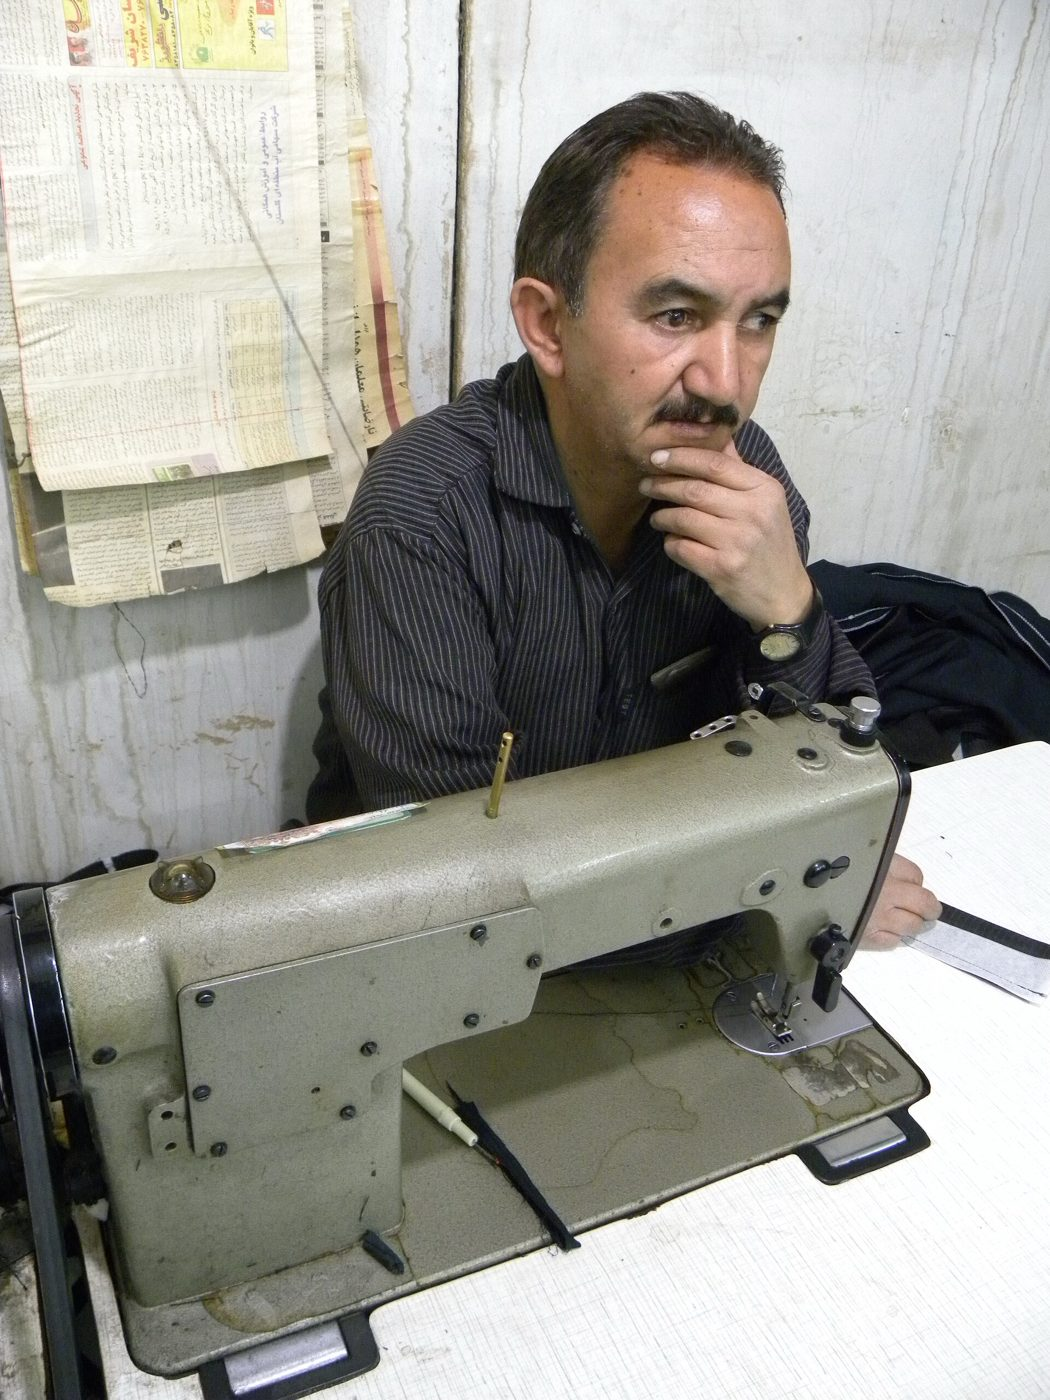
\includegraphics[width=0.78\textwidth,height=0.32\textheight,keepaspectratio]{../../resources/intros/UX-06-seamstress.jpg}\\[0.4em]
{\footnotesize Image : Sonia Sevilla / CC0}
\end{center}

À regarder. Les vidéos sont un contexte. Elles ne sont pas le livrable.
\begin{itemize}
\item UX - Introduction \& Quest n°1, 01Edu \url{https://www.youtube.com/watch?v=UbE6WMeuvQg&list=PLHyAJ_GrRtf-RAtfngbRrFh1XDTnyXFDe}
\end{itemize}

\chapter{Exercice 00 : UX VII - Ex 1 - Stratégie UX}
\exnumber{00}
\extitle{UX VII - Ex 1 - Stratégie UX}
\exfiles{ex00/fichier Figma et PDF, nomme Name\_FirstName\_DeliverableName\_Date\_VersionNumber}
\exauthorize{Ceux nommés dans l'exercice}
\makeheaderfiles

\textbf{Contexte :}

Elsa est couturière. Elle fabrique des maillots de bain sur mesure via son compte Instagram. Ça marche bien, sa communauté grandit ainsi que le volume de demandes de clients.

Cependant, elle perd beaucoup de temps à chaque demande. Pour finaliser une commande, elle doit demander la forme du maillot, la taille, les préférences de couleur et le délai de livraison souhaité. En plus de cela, elle doit s'assurer d'avoir assez de temps pour coudre une pièce  ---  chaque pièce nécessite 6 heures.

Pour l'instant, elle ne travaille qu'avec des messages privés mais elle aimerait passer moins de temps sur cette partie.

Vous lui proposez de l'aider à concevoir une solution pour mieux gérer son temps et son atelier. Vous avez 4 jours de travail.

\textbf{Instructions :}

Maintenant que vous avez découvert et pratiqué de nombreux outils du processus de design, organisez un planning pour les 4 prochains jours de travail.

Sélectionnez au moins un outil pour chaque phase, nommez-le, et tenez compte du temps que chaque phase peut nécessiter.

\begin{itemize}
\item Empathie / Recherche utilisateur
\item Définir
\item Problem Statement
\item Idéation
\item Prototype
\item Test
\end{itemize}

\textbf{Livrables :}

\begin{itemize}
\item Un calendrier, en PDF ou sur Figma, du projet, comprenant les jours ouvrés à venir, chaque phase du processus, les principaux outils que vous prévoyez d'utiliser pour chaque phase et le temps que vous prévoyez de consacrer à chaque outil.
\item Déposez le PDF ou le document Figma sur Github, nommé comme suit : « Nom\_Prénom\_NomDuLivrable\_Date\_NumeroDeVersion ». Par exemple, cela peut être nommé « Doe\_John\_MidFiPrototype\_05242024\_V1 ».
\item Ajoutez un titre dans le document.
\item Soignez l'aspect global du document. Il doit être clair, simple et lisible. Vous pouvez regarder canva.com, sans surcharger le dessin de détails.
\end{itemize}

\textbf{Ressource :}

\begin{itemize}
\item Un récapitulatif de tous les outils qui ont été pratiqués \url{https://www.figma.com/file/x0xfoz9TaEDiAfGPFqKJcs/RECAP-UX%2FUI-Program?node-id=0%3A1}. Concentrez-vous sur la partie UX !
\end{itemize}

\textbf{Citations :}

\begin{itemize}
\item Le design a besoin d'échouer. L'échec est même une étape nécessaire, mais idéalement il doit survenir avant le lancement d'un produit, pendant les phases de prototype et de test
\item « La UX Strategy se situe à l'intersection de l'UX et du business. Elle offre bien plus de chances de créer des produits à succès. Elle permet aux équipes de voir la « big picture » pour atteindre les objectifs business dans des conditions d'incertitude » Jamie Levy | UX Strategy: How to Devise Innovative Digital Products That People Want
\item La UX Strategy est la méthode par laquelle vous validez que votre solution résout un problème pour de vrais clients dans un marché dynamique, car le marché évolue constamment.
\end{itemize}


\chapter{Exercice 01 : UX VII - Ex 2 - Empathie}
\exnumber{01}
\extitle{UX VII - Ex 2 - Empathie}
\exfiles{ex01/archive zip, nomme Name\_FirstName\_DeliverableName\_Date\_VersionNumber}
\exauthorize{Ceux nommés dans l'exercice}
\makeheaderfiles

\textbf{Instructions :}

Utilisez au moins un des outils Empathy du processus de design.

\textbf{Livrables :}

\begin{itemize}
\item Un document PDF avec le script du contexte de l'outil
\item Outil complété (scripts des entretiens utilisateurs, résultats d'une analyse quantitative, etc.)
\item Un document PDF avec les apprentissages clés de cette phase
\item Déposez les documents sur Github, dans un zip nommé « ProjectTitle\_Name\_FirstName », et chaque livrable ainsi : « Name\_FirstName\_DeliverableName\_Date\_VersionNumber ». Exemple : « Doe\_John\_MidFiPrototype\_05242024\_V1 ».
\item Ajoutez un titre dans tous les documents écrits.
\item Soignez l'aspect global des livrables. Ils doivent être clairs, simples et lisibles. Vous pouvez regarder canva.com, sans surcharger le dessin de détails.
\end{itemize}

\textbf{Pistes :}

\begin{itemize}
\item Utilisez autant d'outils que nécessaire, et assurez-vous de faire tout le processus en 4 jours ouvrés !
\end{itemize}

\textbf{Critères :}

\begin{itemize}
\item Entretiens utilisateurs
\begin{itemize}
\item Le script est le guide d'entretien. Assurez-vous qu'il y a :
\begin{itemize}
\item l'objectif principal de l'entretien
\item 1 à 3 hypothèses
\item une introduction appropriée qui décrit l'intervieweur et l'objectif de cet entretien
\item 3 à 5 sujets principaux
\item quelques questions de screening (données démographiques)
\item questions ouvertes, max 10
\item un processus en entonnoir (>)
\item une conclusion avec les prochaines étapes et un remerciement.
\end{itemize}
\item L'outil complété est soit :
\begin{itemize}
\item 5 à 10 scripts d'utilisateurs
\item ou un diagramme d'affinité \url{https://www.youtube.com/watch?v=VngWHIE4k9s} avec les éléments principaux
\end{itemize}
\end{itemize}
\end{itemize}

\begin{itemize}
\item Analytique
\begin{itemize}
\item Le script est le formulaire. Assurez-vous qu'il y a :
\begin{itemize}
\item L'objectif principal du formulaire
\item 1 à 3 hypothèses
\item Une introduction correcte qui décrit l'intervieweur et le but de cet entretien
\item 3 à 5 sujets principaux
\item Quelques questions de filtrage (données démographiques)
\item Questions fermées, sans biais, 10 max
\item Un processus en entonnoir (>)
\item Une conclusion avec les prochaines étapes et un remerciement.
\item Une stratégie de diffusion
\end{itemize}
\item L'outil complété est une série de données quantitatives à partir d'au moins 100 réponses.
\end{itemize}
\end{itemize}

\begin{itemize}
\item Analyse concurrentielle
\begin{itemize}
\item Le script est la stratégie. L'étudiant explique ce qu'il cherche et comment il prévoit de le trouver.
\item L'outil complété est un rapport. Assurez-vous qu'il y a ;
\begin{itemize}
\item Il y a une introduction
\item Il y a un paysage concurrentiel \url{https://venngage-wordpress.s3.amazonaws.com/uploads/2019/03/g2crowd-grid.png}
\item Avec 2 axes pertinents
\item 10 organisations apparaissent sur le paysage concurrentiel
\item Il y a un tableau concurrentiel \url{https://venngage-wordpress.s3.amazonaws.com/uploads/2019/03/product-features-comparison-matrix.png}
\item Avec 5 à 10 critères
\item 10 organisations apparaissent dans le tableau
\end{itemize}
\end{itemize}
\end{itemize}


\chapter{Exercice 02 : UX VII - Ex 3 - Définir}
\exnumber{02}
\extitle{UX VII - Ex 3 - Définir}
\exfiles{ex02/archive zip, nomme Name\_FirstName\_DeliverableName\_Date\_VersionNumber}
\exauthorize{Those named in the exercise}
\makeheaderfiles

\textbf{Instructions :}

Run at least one of the Define tools in the design process.

\textbf{Livrables :}

\begin{itemize}
\item A PDF document with the script of the tool context
\item Completed tool (scripts from user interviews, results from a quantitative analysis, etc.)
\item A PDF document with the key learnings from this phase
\item Déposez les documents sur Github, dans un zip nommé « ProjectTitle\_Name\_FirstName », et chaque livrable ainsi : « Name\_FirstName\_DeliverableName\_Date\_VersionNumber ». Exemple : « Doe\_John\_MidFiPrototype\_05242024\_V1 ».
\item Ajoutez un titre dans tous les documents écrits.
\item Soignez l'aspect global des livrables. Ils doivent être clairs, simples et lisibles. Vous pouvez regarder canva.com, sans surcharger le dessin de détails.
\end{itemize}

\textbf{Pistes :}

\begin{itemize}
\item Use as many tools as needed, be make sure you do all the process in 4 working days!
\end{itemize}

\textbf{Critères :}

\begin{itemize}
\item Persona
\begin{itemize}
\item The script is the list of insights the students uses to create the persona
\item The completed tool is a Persona board \url{https://miro.medium.com/max/1400/0*RbHfR6BHhhFIENNf}. Make sure the key insights come from the field, from reality, but the persona itself is different from only one user.
\end{itemize}
\end{itemize}

\begin{itemize}
\item Empathy Map
\begin{itemize}
\item The script is the list of insights the student uses to create the Empathy map
\item The completed tool is an Empathy Map \url{https://miro.medium.com/max/700/1*I1ffOWdPWQva3dCMQE-TAQ.png}.
\end{itemize}
\end{itemize}

\begin{itemize}
\item User Journey
\begin{itemize}
\item The script is the list of insights the student uses to create the User Journey.
\item The completed tool is a User Journey Map \url{https://d2slcw3kip6qmk.cloudfront.net/marketing/blog/2017Q3/SEO-initiative-customer-journey-mapping/CustomerJourneyMap1.png}.
\end{itemize}
\end{itemize}

\begin{itemize}
\item Jobs-to-be-done (JTBD)
\begin{itemize}
\item The JTBD is tool that goes as a conclusion to another of the previous tools. Make sure:
\begin{itemize}
\item The sentence is complete
\item The "When" part involves a visit on the website
\item The "I want to" part involves a practical action
\item The "So I can" part involves a psychological or emotional purpose
\end{itemize}
\end{itemize}
\end{itemize}


\chapter{Exercice 03 : UX VII - Ex 4 - Énoncé du problème}
\exnumber{03}
\extitle{UX VII - Ex 4 - Énoncé du problème}
\exfiles{ex03/PDF, nomme Name\_FirstName\_DeliverableName\_Date\_VersionNumber}
\exauthorize{Those named in the exercise}
\makeheaderfiles

\textbf{Instructions :}

Based on your research (Empathy \& Define), define a problem statement to narrow the problem and KPIs to measure the success.

\textbf{Livrables :}

\begin{itemize}
\item A PDF document with:
\begin{itemize}
\item One problem statement
\item 1 to 3 KPIs
\item Key learnings from this phase
\end{itemize}
\item Déposez le PDF sur Github, nommé ainsi : « Name\_FirstName\_DeliverableName\_Date\_VersionNumber ». Exemple : « Doe\_John\_MidFiPrototype\_05242024\_V1 ».
\item Ajoutez un titre dans le document.
\item Soignez l'aspect global du document. Il doit être clair, simple et lisible. Vous pouvez regarder canva.com, sans surcharger le dessin de détails.
\end{itemize}

\textbf{Pistes :}
\begin{itemize}
\item KPIs: check the SMART list \url{https://www.grow.com/blog/how-to-use-smart-goals-to-build-your-kpis}) 
\end{itemize}

\textbf{Citation :}

Design is about solving problems. Fall in Love with the Problem, Not the Solution.

\textbf{Examples of Problem statements:}

\begin{itemize}
\item How might we help Pierre measure and prepare his hydration before a race?
\begin{itemize}
\item Appropriate  --- > The problem statement is narrow enough to be specific for one painpoint, and broad enough to let creativity suggest many options. Also, it takes into accounts some of the key insights from the previous phases.
\end{itemize}
\item How might we make sure Pierre doesn't get dehydrated?
\begin{itemize}
\item Too broad  --- > The problem statement is out of the scope of running, so the solutions cannot be integrated in the specific context of running.
\end{itemize}
\item How might we make sure Pierre drinks the cups that are offered during the race?
\begin{itemize}
\item Too narrow  --- > There are plenty of options to avoid dehydration without drinking the cups that are offered during the race.
\end{itemize}
\item How might we provide Pierre with a drink that contains everything he needs to avoid dehydration?
\begin{itemize}
\item Focused on the solution, not the problem  --- > The problem statement is supposed to rephrase the brief and take into account the insights from the previous phase.
\end{itemize}
\item How might make sure Pierre doesn't get drunk the night before the race?
\begin{itemize}
\item Out of scope  --- > This is not about dehydration, nor about running.
\end{itemize}
\end{itemize}


\chapter{Exercice 04 : UX VII - Ex 5 - Idéation}
\exnumber{04}
\extitle{UX VII - Ex 5 - Idéation}
\exfiles{ex04/fichier Figma et PDF, nomme Name\_FirstName\_DeliverableName\_Date\_VersionNumber}
\exauthorize{Those named in the exercise}
\makeheaderfiles

\textbf{Instructions :}

Run at least one of the Ideation techniques in the design process.

\textbf{Livrables :}

\begin{itemize}
\item A PDF document with the script of the tool context
\item Completed tool: a board with all the ideas - on paper or digitally on Miro or Figma
\item A PDF document with the key learnings from this phase
\item Déposez les documents sur Github, dans un zip nommé « ProjectTitle\_Name\_FirstName », et chaque livrable ainsi : « Name\_FirstName\_DeliverableName\_Date\_VersionNumber ». Exemple : « Doe\_John\_MidFiPrototype\_05242024\_V1 ».
\item Ajoutez un titre dans tous les documents écrits.
\item Soignez l'aspect global des livrables. Ils doivent être clairs, simples et lisibles. Vous pouvez regarder canva.com, sans surcharger le dessin de détails.
\end{itemize}

\textbf{Pistes :}

\begin{itemize}
\item Use as many tools as needed, and make sure you do all the process in 4 working days!
\end{itemize}


\chapter{Exercice 05 : UX VII - Ex 6 - Prototype}
\exnumber{05}
\extitle{UX VII - Ex 6 - Prototype}
\exfiles{ex05/archive zip, nomme Name\_FirstName\_DeliverableName\_Date\_VersionNumber}
\exauthorize{Those named in the exercise}
\makeheaderfiles

\textbf{Instructions :}

Make a prototype including the chosen solution.

\textbf{Livrables :}

\begin{itemize}
\item Pictures of a paper prototype (low-fi)
\item An animated wireframe prototype (mid-fi)
\item Key learnings from this phase
\item Vocabulary
\begin{itemize}
\item Basse fidélité : prototypes papier - exemple \url{https://miro.medium.com/max/1400/1*5nUfqqA2gjdAYHagjbHA5w.jpeg}
\item Moyenne fidélité : wireframes, noir et blanc, seulement les éléments principaux, sur un outil de prototype - exemple \url{https://miro.medium.com/max/1400/1*eGSfaxwYbxUFomYbyO6GWw.png}
\item Haute fidélité : wireframes avec couleur, styles, détails graphiques et micro-interactions - exemple \url{https://miro.medium.com/max/1400/1*Xn0HSKAvhr4TZzC9lN5udw.gif}
\end{itemize}
\item Déposez les documents sur Github, dans un zip nommé « ProjectTitle\_Name\_FirstName », et chaque livrable ainsi : « Name\_FirstName\_DeliverableName\_Date\_VersionNumber ». Exemple : « Doe\_John\_MidFiPrototype\_05242024\_V1 ».
\item Ajoutez un titre dans tous les documents écrits.
\item Soignez l'aspect global des livrables. Ils doivent être clairs, simples et lisibles. Vous pouvez regarder canva.com, sans surcharger le dessin de détails.
\end{itemize}

\textbf{Pistes :}

\begin{itemize}
\item Use as many tools as needed, and make sure you do all the process in 4 working days!
\item You may use Card Sorting and User flows
\end{itemize}

\textbf{Critères :}

\subsubsection*{Criteria}

\begin{itemize}
\item User Flow
\end{itemize}

Make sure for each flow:

\begin{itemize}
\item The user has a specific goal
\item There is a starting point and and ending point - which is the goal of the user
\item There is a series of actions organised in rectangles (actions) or diamond (choice)
\item The actions are linked with arrows
\end{itemize}

\begin{itemize}
\item Card sorting
\end{itemize}

Make sure

\begin{itemize}
\item There is a script including the research goals.
\item The research goals must be close to "rearrange the content"
\item There are pictures of the ongoing workshop
\item There is a new content organization shown in a table with sticky notes (it can be a picture or digital)
\end{itemize}


\chapter{Exercice 06 : UX VII - Ex 7 - Test}
\exnumber{06}
\extitle{UX VII - Ex 7 - Test}
\exfiles{ex06/archive zip, nomme Name\_FirstName\_DeliverableName\_Date\_VersionNumber}
\exauthorize{Those named in the exercise}
\makeheaderfiles

\textbf{Instructions :}

Prepare a testing protocol and run it!

\textbf{Livrables :}

\begin{itemize}
\item A testing protocol script
\item Photos from the tests
\item Key learnings from the tests (5 tests are required)
\item Key learnings from this phase
\item Déposez les documents sur Github, dans un zip nommé « ProjectTitle\_Name\_FirstName », et chaque livrable ainsi : « Name\_FirstName\_DeliverableName\_Date\_VersionNumber ». Exemple : « Doe\_John\_MidFiPrototype\_05242024\_V1 ».
\item Ajoutez un titre dans tous les documents écrits.
\item Soignez l'aspect global des livrables. Ils doivent être clairs, simples et lisibles. Vous pouvez regarder canva.com, sans surcharger le dessin de détails.
\end{itemize}


\end{document}
